%%MAIN: thesis.tex

%%%%% The Problem %%%%% and %%%%% Related Work %%%%%
\chapter{State of the Art in Computer Science Didactics} \label{ch_theory}

Before introducing the product of this thesis in chapter \ref{ch_pa}, we first introduce the problem it should help solve: How abstractions involved in programming are taught.

In detail, we first discuss didactic literature on teaching computer science at high school level, introducing the notions of ``foundational idea'' one of which is a \emph{Sichtenwechsel} -- a change of perspective in a multitier architecture; then we show the relevance and limits of abstractions in programming and motivate why students should look beyond a single abstraction layer in \ref{sc_abstractions}.



\section{Didactic Approaches} \label{sc_didactic}

Traditional introductions into programming focus on a single programming language, its syntax and the available semantics -- introducing them iteratively and practising each element with basic exercises. E.\,g. Hartinger introduces most of Python in this way so that it can later be used for scientific calculations \cite{Har20}. 

This traditional introduction works mainly on the level of the programming language, only barely mentioning a simplified memory model (p.\,31) and binary encoding (pp.\,114--115). Interestingly, it does not assume an IDE (see section \ref{ssc_ides} below), but instead very briefly introduces the command line and the Python REPL. Even though in that way, files are not guaranteed to be UTF-8 encoded (as examples assume, cf. p.\,118), encodings are not mentioned beyond pure ASCII. And the Python interpreter is just in the preface briefly characterized as ``program which translates source code into electronic instructions''\footnote{German original: ''[...] das Programm, das den Programmcode in Elektronik-Anweisungen �bersetzt.''}.

While the needs of academic teaching and the form of semester courses with lectures and separate lab work tends to suggest such an approach, this is not a good fit with suggestions from current didactic literature \cite{Sch11, Mod16} (and even past texts \cite{Doy84}):


\subsection{Foundational Ideas} \label{ssc_fundamentale_ideen}

Schubert and Schwill \cite{Sch11} base their didactic approach around the notion of ``foundational ideas'' derived from Jerome Bruner and Alfred Schreiber. A foundational idea is a concept which is deeply ingrained in a specific subject such as computer science and without which the subject would loose part of its core. Additionally, they ask for a foundational idea to have the following properties (pp.\,62--63):
\begin{itemize}
\item Breadth: the concept is applicable not just in one specific context but can be used more generally.
\item Abundance: The concept can be applied in different ways.
\item Meaning: The concept is meaningful to the learner beyond the scope of a course.
\end{itemize}

In a later refinement, the property of Historical Relevance is added by requiring a foundational idea to also have persisted through time \cite[p.\,17]{Mod16}.

Such foundational ideas are among many others the idea of modularization, the idea of layered archictectures or the idea of encoding information and instructions.

As a consequence, they propose an introduction into programming to use several different programming languages along different paradigma: e.\,g. Prolog as a declarative language (pp.\,91--104) and Python as object oriented language (pp.\,157--185), in order to better teach the foundational idea of `language' and to demonstrate to students already at the level of instructions that the language chosen comes with inherent limitations in expressibility (p.\,154, comparing programming languages with natural languages and referring to Wittgenstein's philosophy of language).


\subsection{\emph{Sichtenwechsel}} \label{ssc_sichtenwechsel}

Consequently, they propose to explicitly discuss the foundational idea of multitier architectures -- and that not only in the context of the networking stack and computer archictecture (pp.\,113--116):

They introduce the notion of \emph{Sichtenwechsel}, a change of perspective with relation to the current layer, which should help students better understand concepts of one layer by inspecting lower layers. As an example, they show a live model of a calculator app whose input is translated to both pseudo code and machine code (p.\,115); an environment for inspecting live Java objects (pp.\,208--209); or the Filius environment for inspecting a virtual computer network at its different layers (p.\,284).

They conclude that ``it was a fallacy to assume that students would be able to develop a working model of a computer [...] by designing small programs'' (p.\,213),\footnote{German original: ''Es erwies sich als Irrtum, dass Sch�ler beim Entwerfen kleiner Programme ein tragf�higes kognitives Modell vom Rechner oder von Informatiksystemen im Allgemeinen entwickeln.''} reinforcing the need for going beyond of what traditional programming courses (used to) do.

This conclusion is repeated again and again, e.\,g. by Jaokar \cite[p.\,51]{Jao12} or Zhang \cite[p.\,407]{Zha19}.


\subsection{Manageability} \label{ssc_manageability}

Modrow and Strecker \cite{Mod16} follow Schubert and Schwill \cite{Sch11} in also building upon the concept of foundational ideas. They do however propose to significantly reduce their number and focus on a few very general such ideas such as modelling (\emph{Modellierbarkeit}), connectivity (\emph{Vernetzbarkeit}), digitization (\emph{Digitalisierbarkeit}) and algorithms (\emph{Algorithmisierbarkeit}) (pp.\,27--37). As a consequence, they do propose to focus programming exposure for high school students to block based programming languages such as MIT's Scratch \cite{Mit25} or Berkeley's variant Snap! \cite{Ber25} (p.\,125).

Their reasoning for this is that students should not (yet) have to deal with syntax errors (as opposed to teaching them as suggested by Bouvier \emph{et al.} \cite{Bou24}) and only have a manageable command palette. Furthermore, they note that block based languages with free form layouting encourages to build complex behavior from simple building blocks which can always be run and inspected individually (pp.\,184--185). This allows for a bottom up development approach in which abstractions are incrementally developed out of basic command blocks which they deem more suiteable for students than starting development at the abstract algorithm.

While Modrow and Strecker do suggest also including digital circuits in the curriculum as concrete examples of digitization (p.\,118), they seem content in programming them without inspecting the layers in between. From their foundational idea of connectivity, treating these layers could however still follow: If students are to see how hardware and software are connected -- and that such a connection is even possible --, intermediary steps between program and hardware must be explorable by students.

Following in these footsteps, Chiodini \emph{et al.} \cite{Chi23} similarly state as requirements for programming classes:
\begin{itemize}
\item Manageable complexity: IDEs and APIs must not be unnecessarily complex so as to not confuse students.
\item Meaningful engagement: Samples and exercises should be introduced such that it's clear what they refer to outside of class. Their usefulness shouldn't end at the exam.
\item Clean problem decomposition: Bottom up development should be effortless and code should compose with as little refactoring as possible.
\end{itemize}

The last point explicitly asks for a clean separation of abstraction levels which might be an ideal to strive for but might not be realistically achievable (cf. \ref{ssc_leaky_abstractions}).


\subsection{Teaching Bottom Up} \label{ssc_bottom_up}

Beyond suggesting to connect multiple abstraction layers in a \emph{Sichtenwechsel} (see \ref{ssc_sichtenwechsel}), general didactic literature does not offer more specific suggestions. There are however two readily available ways to deal with abstraction layers: Either starting at the bottom and building abstractions on top; or starting at the most abstract and disecting it into its more fundamental forms.

Starting at the bottom conceptually seems to be the more sound way and is e.\,g. how Mathematics are taught. One rigorous implementation of this approach is offered by Nisan and Schocken \cite{Nis21}: They offer a course which starts with basic logic gates and builds out of them first the parts of and later a fully functioning, basic CPU for which they continue to develop a low level and a high level programming language until reaching the point where applications can be run on the developed hardware (this was originally dubbed as ``NAND to Tetris'').

Their motivation is the same as the motivation for this thesis: ``The most fundamental ideas [...] are now hidden under many layers of obscure interfaces'' (p.\,ix). Since the course is taught at university with hundreds of students, once concession is hardware virtualization: The original logic gates are not built out of silicon or electronics but instead simulated in a portable Java app. This does allow skipping intermediary steps and allows to start the course at any desired level.

Since working with logic gates without seeing their eventual purpose may lack motivation, the course starts with an overview from the top (pp.\,1--4) which also serves as the table of contents. With this, students keep in sight what they're working towards and can start connecting their own preexisting notions with the new material.


\subsection{Teaching Top Down} \label{ssc_top_down}

An alternative teaching approach starts directly at the students' experience, e.\,g. at gaming \cite{Wei16}, art \cite{Rea14} or even toy houses requiring intruder alerts \cite{Mod16} and starts exposing lower abstraction layers as required for gaining more control (and understanding) and extending available capabilities.

At this point a rather traditional approach starts with games: Weintrop and Wilensky \cite{Wei16} discuss a variety of games where programming plays a role in either shaping an avatar, improving its available actions or make it move altogether. Whereas such games are specifically created as `pedagogical' games, many other games have at least part of their logic implemented in scripting languages such as Lua \cite{Lua25} which allows them to be modified by players. While the content involved is more complex, modifying or creating a game within still popular `Roblox' might be sufficiently motivating.

While gaming works as an approach into programming, it's rarely used for inspecting further layers in an educational context. Motivation for doing so is usually constricted to performance optimizations for game platform developers.

An alternative approach which was originally targetted at art students but works well at high school as well is proposed by Reas and Fry \cite{Rea14}: Starting from visual arts and extending the capabilities of the artist through digital means. While the involved programming language, Processing, will be discussed in its own merit in \ref{sc_processing}, their didactic approach is notable as well:

A work of art on its own is something abstract which can not only be interpreted but also created. For (re)creating it, various painting techniques are needed which can be further broken down to basic movements. At this abstraction layer, they set in with high-level programming primitives for creating basic shapes. This allows them to achieve pleasing visual results with just a few commands and initially barely any programming knowledge. Afterwards, the question as to how to achieve more complex output is naturally motivated by already discussed more complex works of art.

Additionally, as art can be considered as individual expression, the parallel to programming as individual expression (as also proposed by Modrow and Strecker \cite{Mod16}) and programming as art is easily drawn: ``To use a tool on a computer, you need do little more than point and click; to create a tool, you must understand the arcane art of computer programming.'' (p.\,3). Finally, programmed art must not remain purely digital and can be extended into physical sculptures, for which at least some considerations about hardware can be introduced.

While in both approaches -- gaming and art --, stepping further down to lower abstraction levels is a possibility, only one or two such steps are naturally motivated from the source material. Nonetheless, in both cases a \emph{Sichtenwechsel} is possible.


\subsection{Exploratory and Live Programming} \label{ssc_exploration}

Live programming refers to output and other intermediary products being adapted or recalculated every time source code changes, without any explicit saving and/or rerunning required by the programmer \cite{Rei18}. This gives students the quickest results, as otherwise they might tend to work on code too long without occasionally testing it, if doing so requires additional interactions (for the same reason, many applications have switched to auto-saving instead of relying on users to do so manually from time to time). Live programming also gives students immediate feedback about their code and modifications.

Exploratory programming on the other hand refers to students being given sample code and then modifying said code in order to figure out what effects their modifications have, building like this a mental model of what the code performs.

Both Schubert and Schwill \cite[p.\,367]{Sch11} and Modrow and Strecker \cite[p.\,167]{Mod16} suggest exploratory programming for allowing students to work at their own speed and depth: With given examples, less experienced students can stay closer to the given -- simple but working -- code, while more experienced students can use their knowledge for testing more complicated hypotheses.

While live programming requires explicit support from the programming environment (see \ref{ssc_ides}), exploratory programming can be done without. Apps can still support exploration better by providing a form of REPL\footnote{REPL is short for \emph{Read-Evaluate-Print-Loop} i.\,e. an interactive interpreter.} which most scripting languages do, an interactive notebook (such as Jupyter or Lepiter, see \ref{sc_gt}) or a way of direclty running any part of a program, as Scratch does (see \ref{ssc_manageability}).

The didactic reasons for using both exploratory and live programming also apply outside or pure programming, such as when inspecting and modifying live systems, networks, \emph{etc.}.


\subsection{Computational Thinking} \label{ssc_ct}

Since other disciplines have started to rely on computers as more than a glorified typewriter and filing system, the notion of preparing students for working in academia and industry has shifted from teaching applications to teaching ``Computational Thinking''. Lee \emph{et al.} \cite{Lee20} have assembled cases from schools where programming is used in physics, biology, chemistry and other sciences, linking it to the role that mathematics have had in the past centuries.

As a basis for employing programming, simulation or data transformations to solve problems in other domains, students must be versed in dealing with different abstraction levels in order to connect the abilities of a computer with the subject at hand. Buitrago \emph{et al.} \cite{Bui17} also point out that students must know the limits of computers and not attribute them understanding and intelligence.

With the sudden rise of large language models in the past decade, computational thinking even refers back to programming: Martini \cite{Mar24} argues that with LLMs being able to write programs on their own, programming curricula have to be adjusted accordingly. Students will still have to be able to understand the basics, in order to be able to instruct an LLM towards a desired result.

Also, recent studies seem to suggest that relying on LLMs for coding does not lead to better developer performance \cite{Bec25} nor to better code \cite{Moh25}, as cognitive offloading has been observed. This effect is likely even more pronounced for students, as getting quick results for simple tasks might lull them into overconfidence with relation to the available LLM.

As a consequence, the functioning and limits of large language models must not only be taught as part of computational thinking but also used as another example for examining different abstraction levels in a computer system.



\section{Multitier Architectures / Abstractions} \label{sc_abstractions}

In order to handle complexities arising in both theoretical and practical computer science, subjects are split into multiple layers or tiers to be described, investigated and used separatedly.

Common such multitier architectures taught at high school level are the networking stack (either the seven layered OSI model or the simplified four layered DoD architecture) or the software-hardware stack ranging from apps and hardware abstracting OS down to transistors consisting of e.\,g. silicium atoms (see figure \ref{fig_multitier}).

\begin{figure} \label{fig_multitier}
\centering
% adapted from https://github.com/dev-gb/TikZ-osi-model
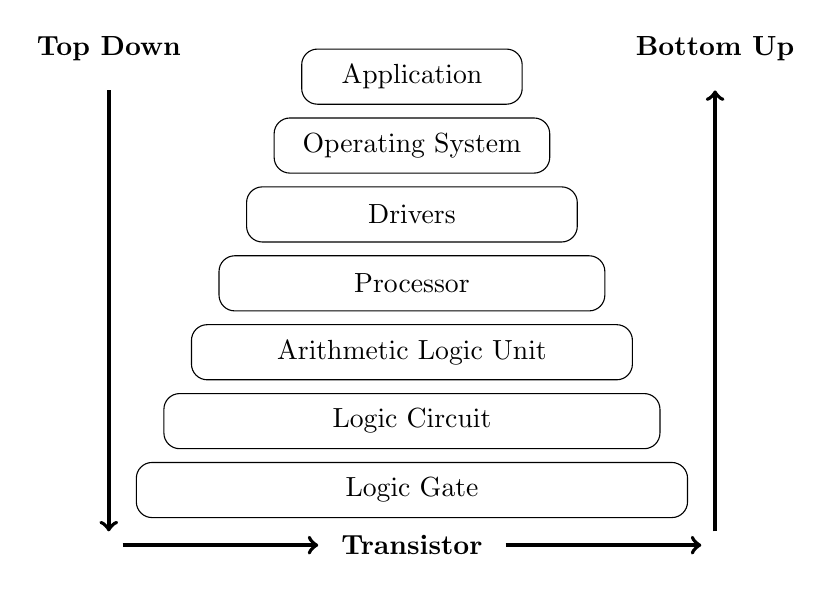
\begin{tikzpicture}[scale=0.7]

\draw[rounded corners=2mm] (-2,0) rectangle (2,-1);
\draw[rounded corners=2mm] (-2.5,-1.25) rectangle (2.5,-2.25);
\draw[rounded corners=2mm] (-3,-2.5) rectangle (3,-3.5);
\draw[rounded corners=2mm] (-3.5,-3.75) rectangle (3.5,-4.75);
\draw[rounded corners=2mm] (-4,-5) rectangle (4,-6);
\draw[rounded corners=2mm] (-4.5,-6.25) rectangle (4.5,-7.25);
\draw[rounded corners=2mm] (-5,-7.5) rectangle (5,-8.5);

\node at (0, -0.5) {Application};
\node at (0, -1.75) {Operating System};
\node at (0, -3) {Drivers};
\node at (0, -4.25) {Processor};
\node at (0, -5.5) {Arithmetic Logic Unit};
\node at (0, -6.75) {Logic Circuit};
\node at (0, -8) {Logic Gate};

\node[align = center] at (-5.5, 0) {\textbf{Top Down}};
\node[align = center] at (5.5, 0) {\textbf{Bottom Up}};
\node at (0, -9) {\textbf{Transistor}};

\draw[->, line width=0.5mm] (-5.5,-0.75) -- (-5.5,-8.75);
\draw[->, line width=0.5mm] (-5.25,-9) -- (-1.7,-9);
\draw[->, line width=0.5mm] (1.7,-9) -- (5.25,-9);
\draw[->, line width=0.5mm] (5.5,-8.75) -- (5.5,-0.75);

\end{tikzpicture}
\lessSpace
\caption{Multitier model of a computer system.}
\end{figure}

Ideally, in such architectures all layers above the layer to be investigated can be ignored (beyond what the layer will be used for) and all the layers below can be abstracted away into a nicely defined interface.

As such, programming should be possible to be done independently of hardware and even the operating system, in the same way that natural languages can be taught independently of body or mind of the students.

This analogy however shows that even in computer science, the philosophical mind-body problem persists, albeit in a different form: ``At the grossest physical level, a computer process is a series of changes in the state of a machine'' \cite[p.\,12]{Col99}. In contrast to the human mind, where the interaction between objectively observable brain matter and subjective thought is at the core of an ongoing philosophical and neuroscientific debate, in computer science this duality of having electrical currenty on the one hand and a running program on the other is decomposable all the way through.

And as has been shown in \ref{sc_didactic}, didactic literature suggests that this feature should be discussed, as this is a foundational idea of computer science.


\subsection{Leaky Abstractions} \label{ssc_leaky_abstractions}

In his article ``The Law of Leaky Abstractions'' \cite{Spo02} introduces the concept of \emph{leaky abstractions}, claiming that for all non-trivial such architectures, details of lower layers are to some degree bound to bleed through to upper layers. In other words, in practice complex interfaces tend to be incomplete or 'leaky'.

In teaching computer science, such leaky abstractions occur repeatedly, e.\,g. when an app doesn't run on a different device (with either the OS or the processor architecture leaking); or when a document seemingly can't be saved (with either the file system or differences between apps leaking).

More specifically, in programming there are several ways of abstracting away technical details:

\begin{itemize}
\item Programming instructions consist of source code which consists of encoded bits which are stored in memory or on a drive.
\item Source code consists of tokens which are usually parsed into an abstract syntax tree (AST) which are either directly or via intermediary representations translated into machine code to be run on a virtual or actual machine.
\item When programming instructions through the above abstractions are executed, variable values are encoded and stored in memory, function calls are tracked through a call stack, input state is continually mapped into memory and output is generated in several forms -- where e.\,g. textual output causes a font renderer to interpret glyph instructions for every character; or graphical output is anti-aliased before any pixel data is produced.
\end{itemize}

Of these different layers, students usually focus on turining instructions into source code and then checking the program's output -- or any error messages produced by the compiler or interpreter (see section \ref{sc_didactic}). Still, several of the lower layered abstractions might leak through, such as:

\begin{itemize}
\item Missing a stop condition in a recursive function leads to a cryptic ``Stack overflow'' error -- leaking information about the call stack.
\item If a program outputs emojis, they might look notably differently in source code and output -- leaking font rendering.
\item Similarly, programs containing emojis might have emojis garbled depending on the app used for inspecting the source code -- leaking text encoding.
\item If a program contains an endless loop, there might be neither error message nor output, so that it might wrongly seem that the computer isn't doing anything. This isn't an abstraction leak in the above sense but a related student misconception.
\end{itemize}

Besides the above rather easily observable abstraction leaks, the issue might also have to be discussed itself, since recently one class of leaky abstractions has been shown to be security critical: timing attacks. Since programs might be compiled differently and optimized differently and run on different hardware, runtime timing is not considered to be inherent to a particular source code.\footnote{At least beyond generic complexity considerations on an algorithmic level.}

In cryptography, timing attacks have been successfully used for extracting passwords from insufficiently protected webservers \cite{Por18}. More recently, another class of timing attacks taking advantage of modern CPU's branch prediction optimizations has been demonstrated \cite{Koc19}. In the latter case, an implementation detail of the CPU managed to leak. And in both cases, at least implementors of cryptographic programs must be aware of lower abstraction layers.

Further examples of leaky abstractions are discussed by Egger \cite{Egg24} and many others \cite{Nat25, Kan25}. These show that knowledge of lower layers are particularly important for developers of compilers and other performance-critical programs: In order to optimize a program, the specifics of the platform architecture and the implementation of processors and networking become crucial.

Since abstraction leaks are unavoidable in programming -- even with block based languages such as Scratch --, they have to be discussed anyway. Instead of tackling them one by one as separate exceptional cases, literature discussed above suggests to use this opportunity to work out the foundational idea of a multitier architecture and of the interconnectivity of computer systems.


\subsection{Abstractions in IDEs} \label{ssc_ides}

Integrated development environments used for programming offer a variety of different views on a program beyond its source code and its runtime output. The popular Visual Studio Code offers e.\,g. through extensions step-by-step debugging with variables and the call stack listed \cite{Mic25}. This is mirrored in most other full fledged IDEs such as PyCharm \cite{Jet25} or Eclipse \cite{Ecl25}.

And while such IDEs through appropriate extensions even allow inspecting Python bytecode, the respective views are usually overwhelming for programming novices and thus rather targetted at professional developers than high school students.

As a remedy, several teaching oriented IDEs have been developped, such as ``Code with Mu'' which offers a minimal command set and still allows runtime inspection \cite{Tol23}; or Thonny which had the goal to visualize runtime concepts beyond what IDEs offered at the time \cite[p.\,119]{Ann15}:

On the one hand, Thonny shows intermediary steps during expression evaluation. This demonstrates that statements are not evaluated in one go, but indeed in a predetermined order operation by operation.\footnote{In professional IDEs, intermediary results are usually available by hovering over a specific operator with the order of evaluation being left to the user to determine.}

On the other hand, Thonny visualizes recursion by showing code in a new pop-up for every function call, so that multiple recursive function calls lead to an equivalent number of visible pop-ups. Most other IDEs rather show a call stack as in a separate view, which abstracts the stack into a list.\footnote{As a compromise, Glamorous Toolkit presented in chapter \ref{ch_background} displays the call stack as a list of expandable method sources with the call location highlighted.}

Finally, Thonny distinguishes between values on the stack and on the heap, showing the pointer to the heap as the value actually pushed on the stack and in a separate view the actual object on the heap at the given address.

Thus, the Thonny IDE set out to and indeed nicely visualizes several concepts on lower runtime layers.

Jalalitabar and Wang \cite{Jal22} have assembled a list of tools targetted at visualizing some of these concepts outside of an IDE. One noteable such alternative approach is taken by Python Tutor \cite{Pyt25} which combines a visualization of stack frames variable values as pointers and deconstructed objects.

Sychev \cite{Syc21} suggests as an additional IDE feature hints for syntax errors which show students a side-by-side view of their entered code and the corrected code with all required transformations highlighted. They have implemented this feature for Moodle.

Bouvier \emph{et al.} \cite{Bou24} ask for an extension of this: a view to show details about any form of errors, helping students to better understand the issue at hand. In particular, they suggest including an LLM assistant which can further help explain an error to a novice student. How effective such an assistant would be, remains to be seen (see \ref{ssc_ct}).

Comparing to programming IDEs, the web development consoles offered by modern web browsers also provide a variety of views into the various layers of the network stack. These views are however tailored to answer the most common questions of a web developer instead of providing a coherent overview of how the network layers interact.

\begin{todo}
\item Conclusion
\end{todo}
